%% Developing a solution for multimedia home networking chapter
%% author Liu Peng

We developed an Android application that has integrated with a simple media server, 
Airplay/DLNA/Chromecast device discovery, and Airplay/DLNA/Chromecast streaming
control point.

\subsection{Architecture overview}

A simplified version of our implementation is shown in the figure \ref{chart3} below:
\begin{figure}[htb]
\centering 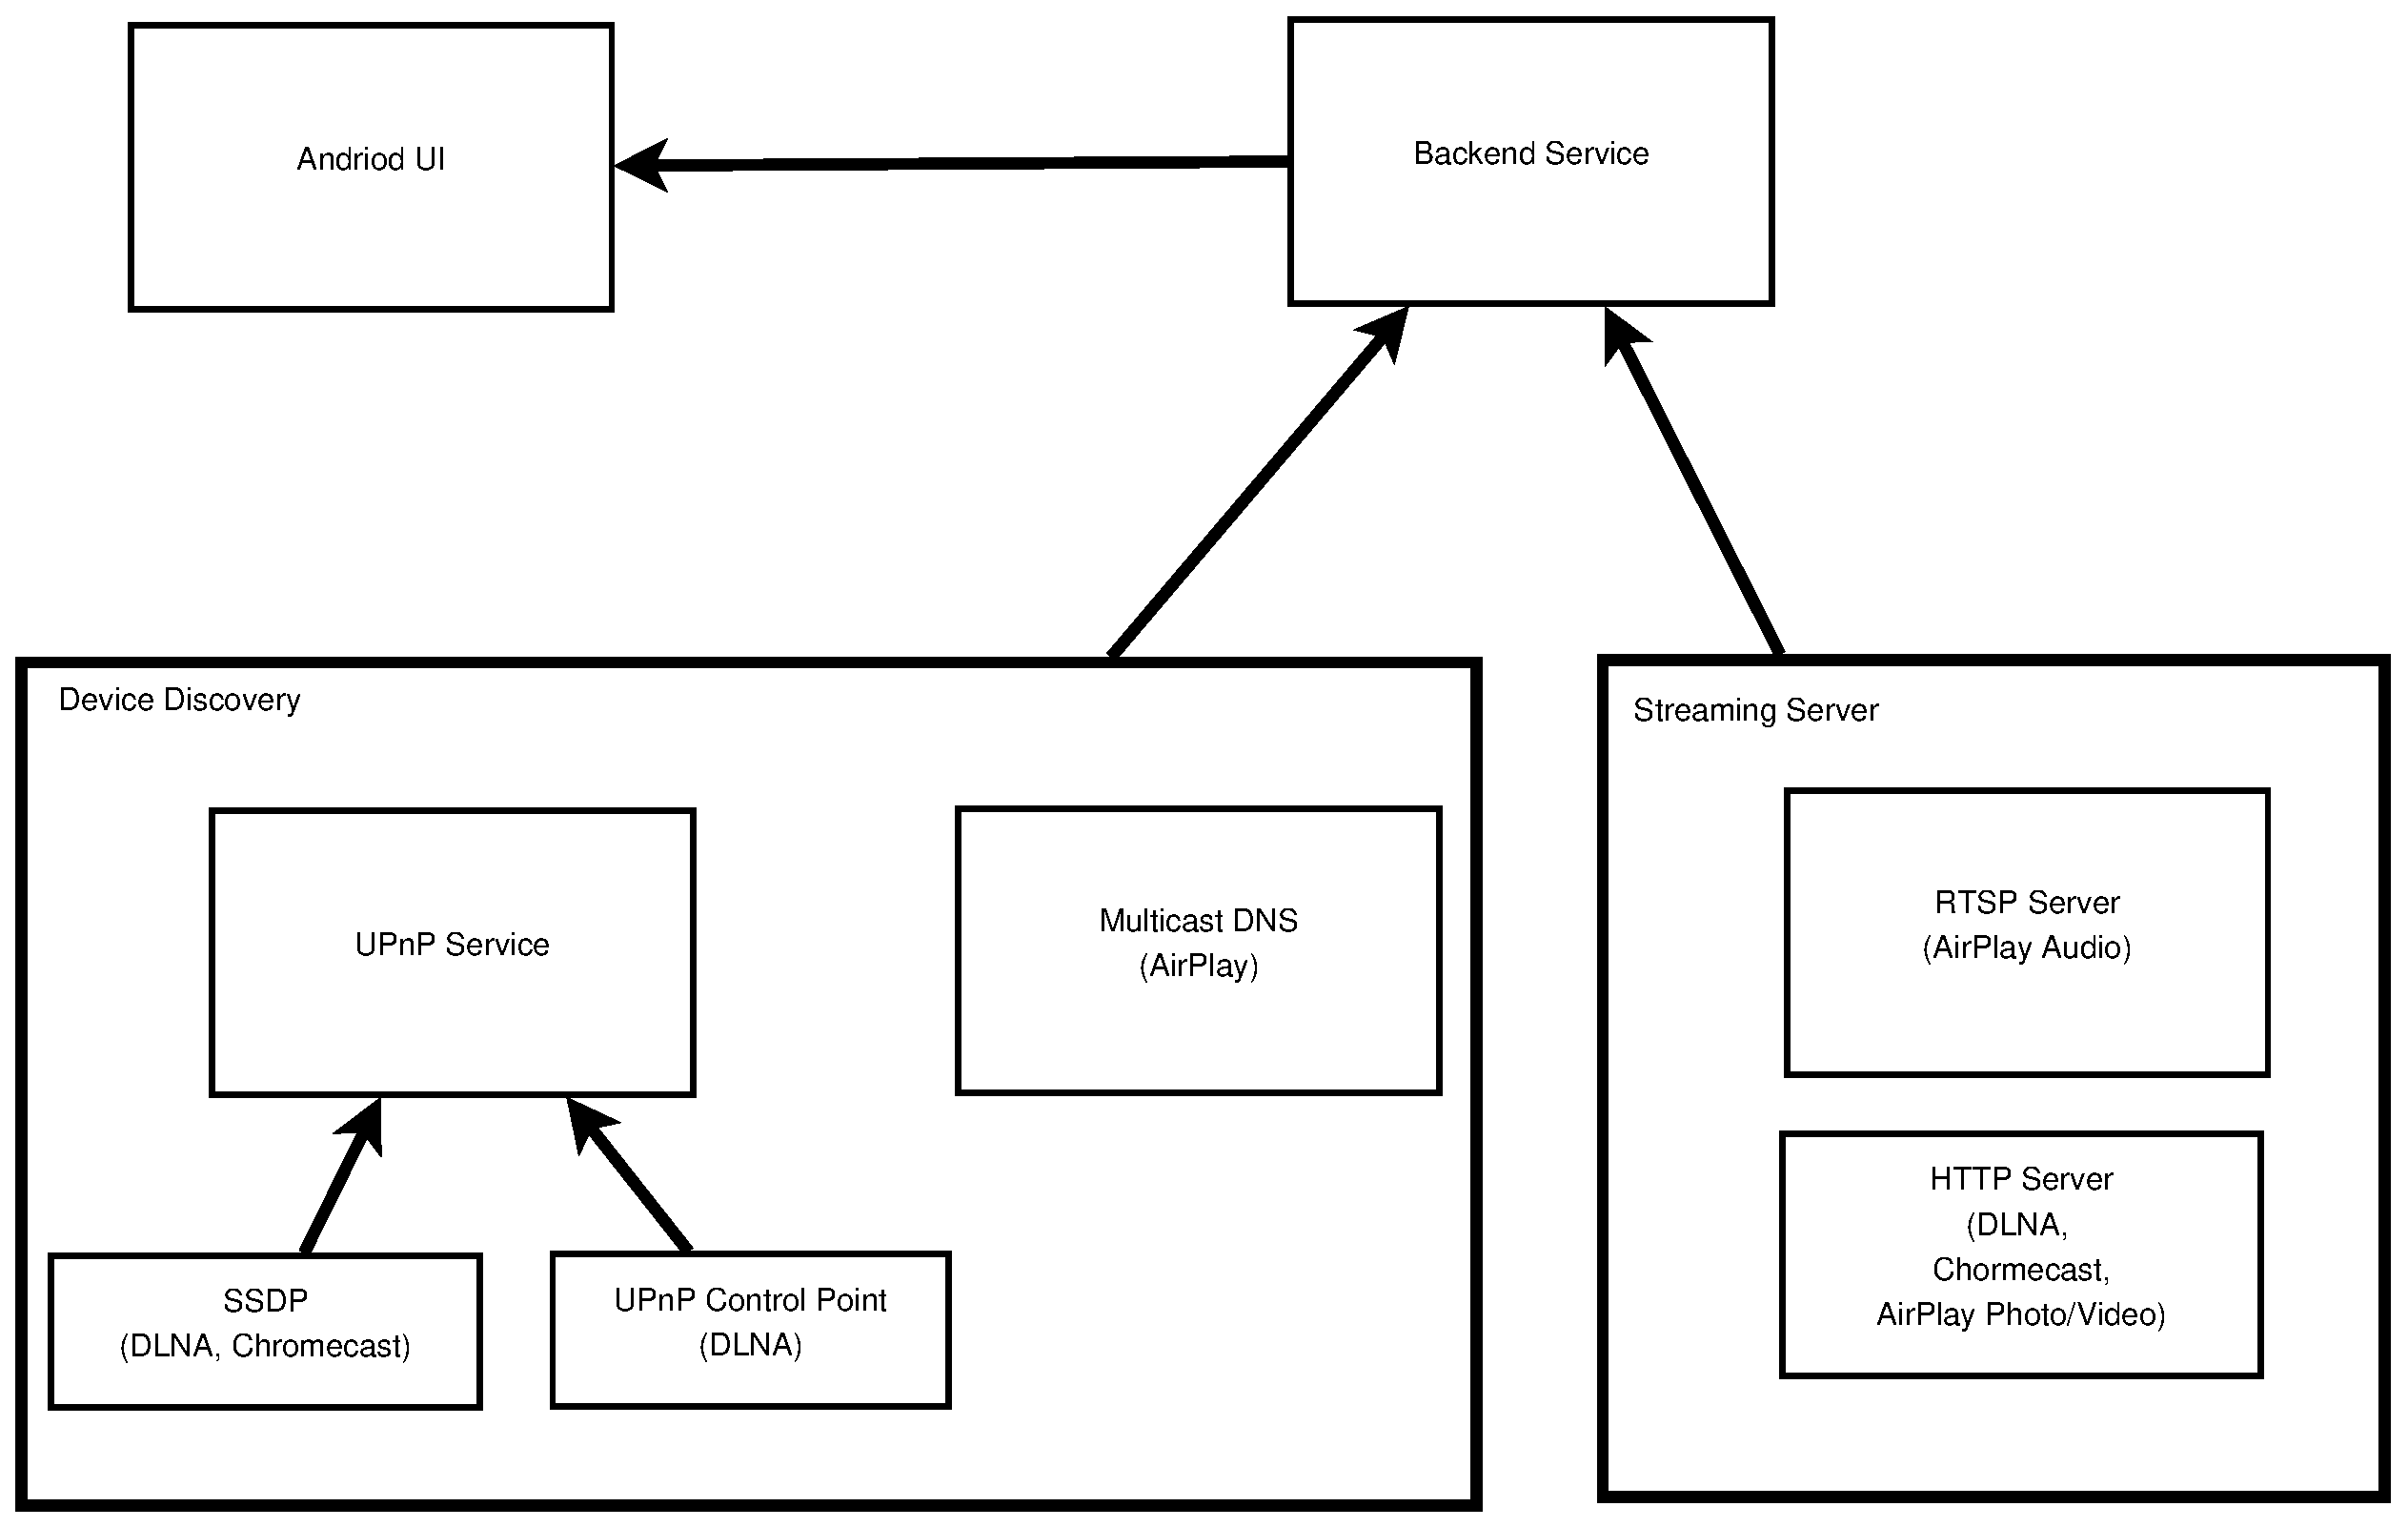
\includegraphics[height=9cm]{charts/chart3}
\caption{Simplified flow chart \label{chart3}}
\end{figure}

\begin{figure}[htb]
\centering 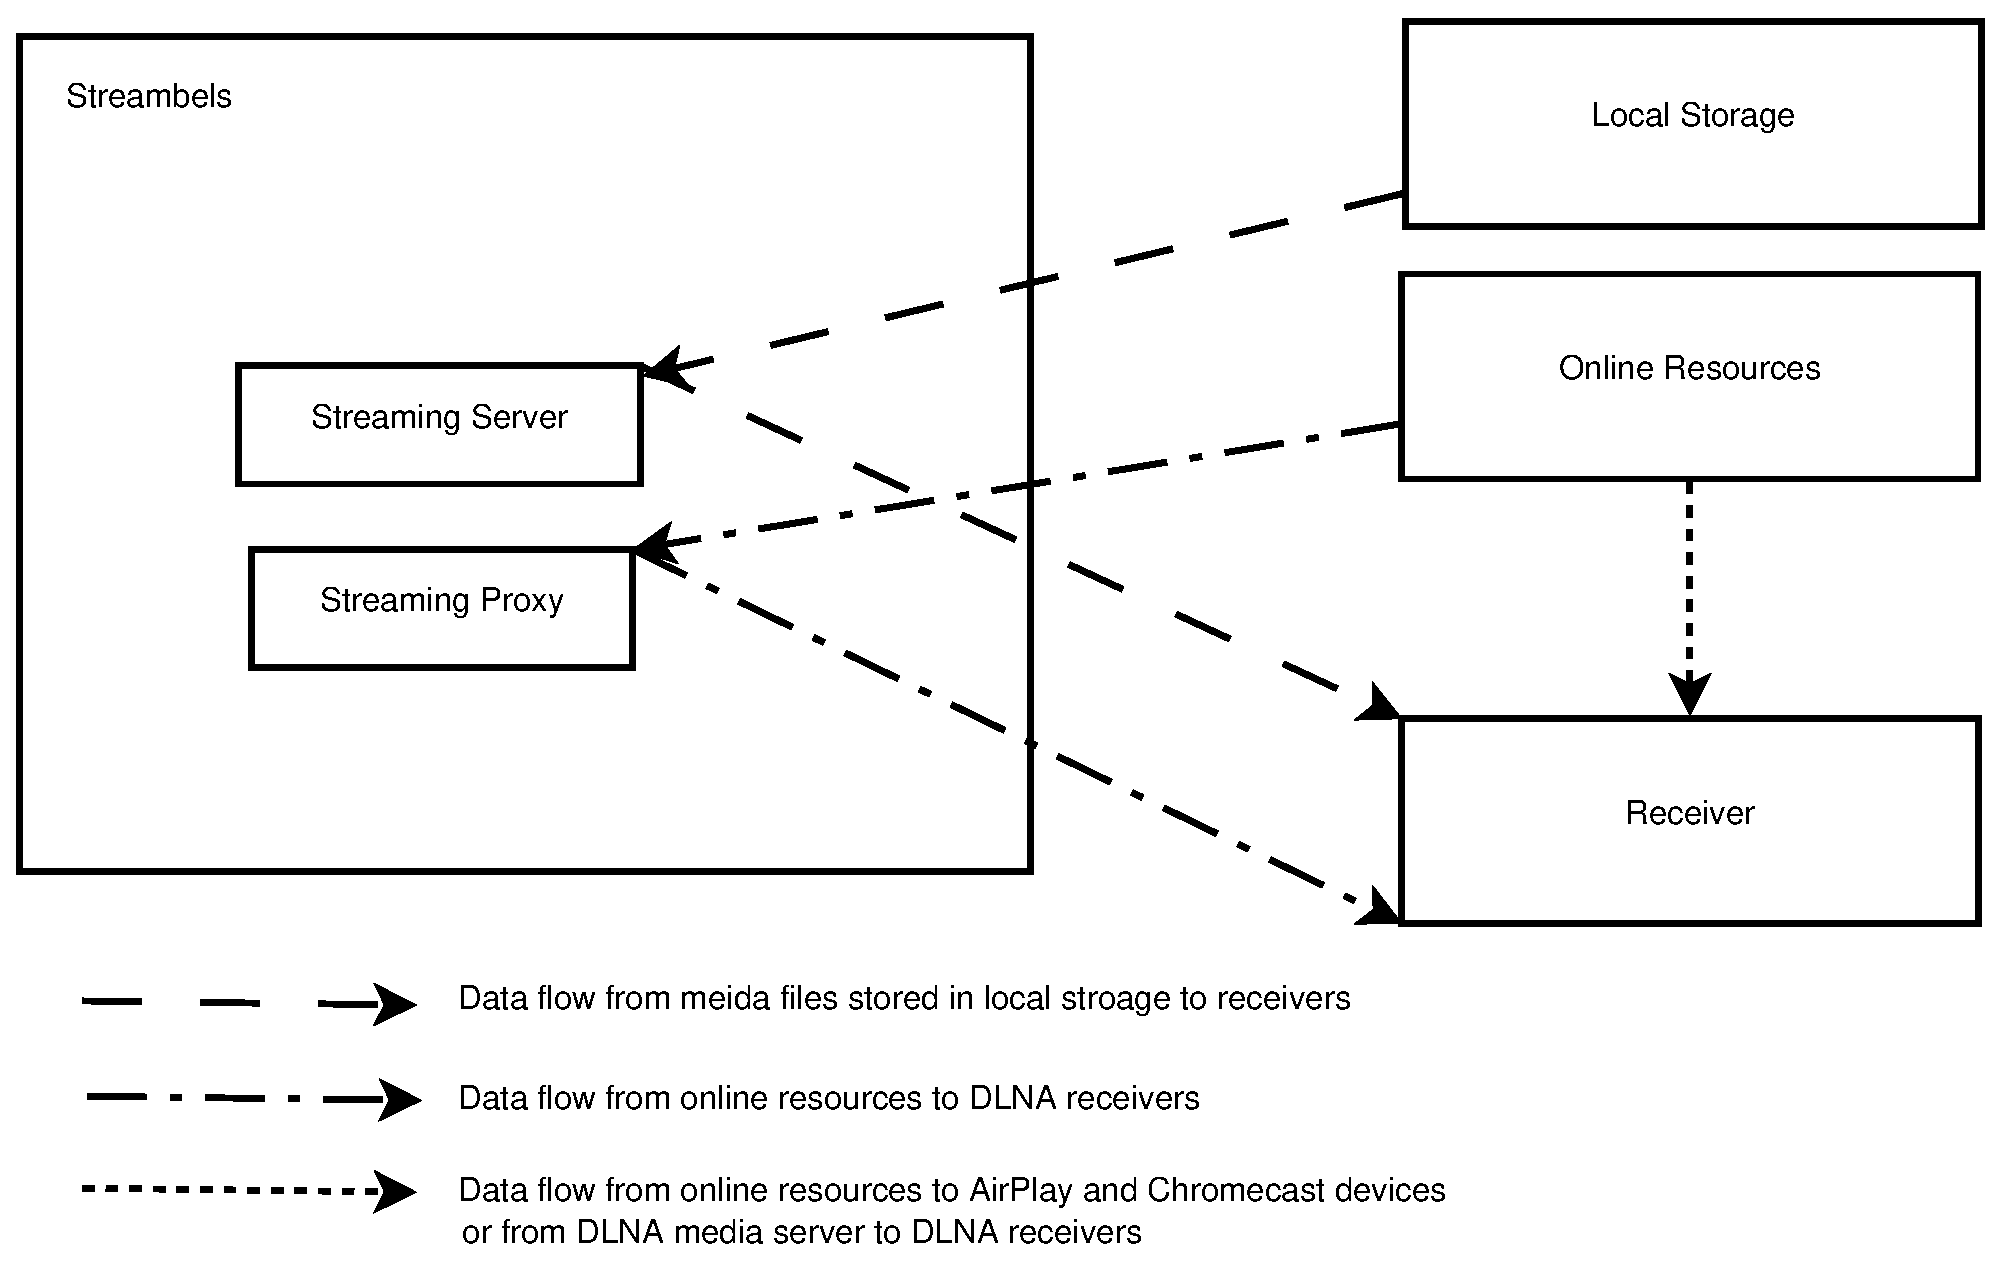
\includegraphics[height=9cm]{charts/data_flow}
\caption{Simplified data flow \label{chart4}}
\end{figure}


\subsection{Features}
As we know that Airplay and DLNA works differently and have different features, but 
according to the previous study, we could combine some use cases of both protocols. 
We are developing an Android application that can handle most multimedia devices in 
a typical home networking. Feature list:
\begin{itemize}
\item[--]Firstly the app is a multimedia player, it can play music, photos and videos 
on SD card locally on Android phone
\item[--]It can stream local content to Apple TV, Airport express and Airplay-enabled 
speakers.
\item[--]It can stream local content to DLNA media renderers, which has a huge device 
base.
\item[--]It can stream local content to Chromecast devices.
\item[--]It can browse content from the DLNA media servers, a typical source is a 
Network Attached Storage (NAS). And play the media locally on the Android device.
\item[--]It can browse content from the DLNA media servers and stream it to DLNA media 
renderers.
\item[--]It can browse content from DLNA media servers and stream it to Airplay enabled 
devices using a different protocol.
\item[--]It can proxy online channels' content to DLNA and Airplay enabled devices. 
(Currently YouTube and Facebook videos are supported, but integration to Spotify is still 
in progress).
\end{itemize}

\subsection{Extensibility}
In normal use cases, the data flow can be shown as figure \ref{chart4},
Streambels has embedded a media streaming server for local files and streaming
proxy. By using built-in proxy, Streambels is able to share online resources
from Internet to devices in home networking environment. New services and new
content providers can be easily added by just call the proxy interface.

The proxy system enables a huge extensibility possibility, which connects the
home networking and Internet.

\subsection{Evaluation methodology}
Since the project is targeted to Android market, and is directly used by
end-users, feedback is really important to us for the continuous development. We
used Email for normal communication, user can edit feedback content directly
inside the application, and later content is sent to us by email.

There is no perfect application, so crash sometimes happen, thanks to Google,
the Google will help to collect the crash reports and show it inside developer
console.

Inside Streambels, we also used Google's Analytics API, which give us
great convinience to collect number of users and sessions every day. Other
information like operation system version, application version, active users
helped us to have insights into who are our users and how can we market for more
people in the world.

It is also interesting to see what kind of technologies are most used in their
daily life, thanks to Google's analytics SDK, we can trigger events when user
selected their receivers, so after months of statistics, we can figure out the
most popular standards and most popular online channels that user uses.


